% answers.tex —— 2003 年·辽宁卷 · 参考答案与详细解析片段
% 由 tools/generate_projects.py 依来源总账自 2003/2003_数学真题_辽宁_试题.md + 2003/2003_数学真题_辽宁_解析正文.md + 2003/2003_数学真题_辽宁_答案要点.md 生成，勿手改（改源 MD 后重跑）


\begin{gktip}
固定源 PDF 仅含 2 页题面，无官方答案与解析页。以下各题均依据题面独立复算并经双角色交叉核验；第 15、17 题的图形在 LaTeX 工程中统一采用 TikZ 矢量重绘。
\end{gktip}

\begin{answer}
\gksolhead{1}{}

\textbf{题目}：

与曲线 $y = \dfrac{1}{x-1}$ 关于原点对称的曲线为\mbox{（　　）}

（A）$y = \dfrac{1}{1+x}$　　（B）$y = -\dfrac{1}{1+x}$　　（C）$y = \dfrac{1}{1-x}$　　（D）$y = -\dfrac{1}{1-x}$

\Needspace{4\baselineskip}
\textbf{解析}

曲线关于原点对称，只需将方程中的点 $(x, y)$ 替换为 $(-x, -y)$。
\Needspace{5\baselineskip}
原方程为：
\nopagebreak[4]
\[y = \frac{1}{x - 1}.\]
\Needspace{5\baselineskip}
关于原点对称后的方程为：
\nopagebreak[4]
\[-y = \frac{1}{-x - 1} \implies -y = -\frac{1}{x + 1} \implies y = \frac{1}{x + 1} = \frac{1}{1 + x}.\]

故选 A。

\gkanswer{答案：A}

\end{answer}
\begin{answer}
\gksolhead{2}{}

\textbf{题目}：

已知 $x \in \left(-\dfrac{\pi}{2}, 0\right)$，$\cos x = \dfrac{4}{5}$，则 $\tan 2x =$\mbox{（　　）}

（A）$\dfrac{7}{24}$　　（B）$-\dfrac{7}{24}$　　（C）$\dfrac{24}{7}$　　（D）$-\dfrac{24}{7}$

\Needspace{4\baselineskip}
\textbf{解析}

由 $x \in \left(-\dfrac{\pi}{2}, 0\right)$，可知 $x$ 为第四象限角，$\sin x < 0$。
\Needspace{5\baselineskip}
已知 $\cos x = \dfrac{4}{5}$，则：
\nopagebreak[4]
\[\sin x = -\sqrt{1 - \cos^2 x} = -\sqrt{1 - \left(\frac{4}{5}\right)^2} = -\frac{3}{5}.\]
\Needspace{5\baselineskip}
所以：
\nopagebreak[4]
\[\tan x = \frac{\sin x}{\cos x} = \frac{-3/5}{4/5} = -\frac{3}{4}.\]
\Needspace{5\baselineskip}
利用倍角公式：
\nopagebreak[4]
\[\tan 2x = \frac{2\tan x}{1 - \tan^2 x} = \frac{2 \times \left(-\dfrac{3}{4}\right)}{1 - \left(-\dfrac{3}{4}\right)^2} = \frac{-\dfrac{3}{2}}{1 - \dfrac{9}{16}} = \frac{-\dfrac{3}{2}}{\dfrac{7}{16}} = -\frac{24}{7}.\]

故选 D。

\gkanswer{答案：D}

\end{answer}
\begin{answer}
\gksolhead{3}{}

\textbf{题目}：

$\dfrac{1 - \sqrt{3}\mathrm{i}}{(\sqrt{3} + \mathrm{i})^2} =$\mbox{（　　）}

（A）$\dfrac{1}{4} + \dfrac{\sqrt{3}}{4}\mathrm{i}$　　（B）$-\dfrac{1}{4} - \dfrac{\sqrt{3}}{4}\mathrm{i}$　　（C）$\dfrac{1}{2} + \dfrac{\sqrt{3}}{2}\mathrm{i}$　　（D）$-\dfrac{1}{2} - \dfrac{\sqrt{3}}{2}\mathrm{i}$

\Needspace{4\baselineskip}
\textbf{解析}

\Needspace{5\baselineskip}
先计算分母：
\nopagebreak[4]
\[(\sqrt{3} + \mathrm{i})^2 = (\sqrt{3})^2 + 2\sqrt{3}\mathrm{i} + \mathrm{i}^2 = 3 + 2\sqrt{3}\mathrm{i} - 1 = 2 + 2\sqrt{3}\mathrm{i} = 2(1 + \sqrt{3}\mathrm{i}).\]
\Needspace{5\baselineskip}
代入分式：
\nopagebreak[4]
\[\frac{1 - \sqrt{3}\mathrm{i}}{(\sqrt{3} + \mathrm{i})^2} = \frac{1 - \sqrt{3}\mathrm{i}}{2(1 + \sqrt{3}\mathrm{i})}.\]
\Needspace{5\baselineskip}
分子分母同乘以 $1 - \sqrt{3}\mathrm{i}$：
\nopagebreak[4]
\[\frac{(1 - \sqrt{3}\mathrm{i})^2}{2(1 + \sqrt{3}\mathrm{i})(1 - \sqrt{3}\mathrm{i})} = \frac{1 - 2\sqrt{3}\mathrm{i} + (\sqrt{3}\mathrm{i})^2}{2(1 + 3)} = \frac{1 - 2\sqrt{3}\mathrm{i} - 3}{8} = \frac{-2 - 2\sqrt{3}\mathrm{i}}{8} = -\frac{1}{4} - \frac{\sqrt{3}}{4}\mathrm{i}.\]

故选 B。

\gkanswer{答案：B}

\end{answer}
\begin{answer}
\gksolhead{4}{}

\textbf{题目}：

已知四边形 $ABCD$ 是菱形，点 $P$ 在对角线 $AC$ 上（不包括端点 $A, C$），则 $\vec{AP} =$\mbox{（　　）}

（A）$\lambda(\vec{AB} + \vec{AD})$，$\lambda \in (0, 1)$　　（B）$\lambda(\vec{AB} + \vec{BC})$，$\lambda \in \left(0, \dfrac{\sqrt{2}}{2}\right)$

（C）$\lambda(\vec{AB} - \vec{AD})$，$\lambda \in (0, 1)$　　（D）$\lambda(\vec{AB} - \vec{BC})$，$\lambda \in \left(0, \dfrac{\sqrt{2}}{2}\right)$

\Needspace{4\baselineskip}
\textbf{解析}

\Needspace{5\baselineskip}
在菱形 $ABCD$ 中，根据向量加法的平行四边形法则，对角线向量为：
\nopagebreak[4]
\[\vec{AC} = \vec{AB} + \vec{AD}.\]
因为点 $P$ 在对角线 $AC$ 上，且不包括端点 $A, C$，所以向量 $\vec{AP}$ 与 $\vec{AC}$ 同向共线，且模长满足 $0 < |\vec{AP}| < |\vec{AC}|$。
\Needspace{5\baselineskip}
因此存在唯一的实数 $\lambda \in (0, 1)$，使得：
\nopagebreak[4]
\[\vec{AP} = \lambda \vec{AC} = \lambda(\vec{AB} + \vec{AD}).\]

故选 A。

\gkanswer{答案：A}

\end{answer}
\begin{answer}
\gksolhead{5}{}

\textbf{题目}：

\Needspace{5\baselineskip}
设函数
\nopagebreak[4]
\[f(x) = \begin{cases} 2^{-x} - 1, & x \le 0, \\ x^{\frac{1}{2}}, & x > 0, \end{cases}\]
若 $f(x_0) > 1$，则 $x_0$ 的取值范围是\mbox{（　　）}

（A）$(-1, 1)$　　（B）$(-1, +\infty)$　　（C）$(-\infty, -2) \cup (0, +\infty)$　　（D）$(-\infty, -1) \cup (1, +\infty)$

\Needspace{4\baselineskip}
\textbf{解析}

分段函数 $f(x) = \begin{cases} 2^{-x} - 1, & x \le 0, \\ x^{\frac{1}{2}}, & x > 0. \end{cases}$
要求 $f(x_0) > 1$，分两种情况讨论：
\Needspace{5\baselineskip}
1. 当 $x_0 \le 0$ 时：
\nopagebreak[4]
\[2^{-x_0} - 1 > 1 \iff 2^{-x_0} > 2 \iff -x_0 > 1 \iff x_0 < -1.\]
   因为 $-1 \le 0$，所以此时解为 $x_0 \in (-\infty, -1)$。
\Needspace{5\baselineskip}
2. 当 $x_0 > 0$ 时：
\nopagebreak[4]
\[x_0^{\frac{1}{2}} > 1 \iff \sqrt{x_0} > 1 \iff x_0 > 1.\]
   结合 $x_0 > 0$，此时解为 $x_0 \in (1, +\infty)$。

综合上述两种情形，$x_0$ 的取值范围为 $(-\infty, -1) \cup (1, +\infty)$。

故选 D。

\gkanswer{答案：D}

\end{answer}
\begin{answer}
\gksolhead{6}{}

\textbf{题目}：

等差数列 $\{a_n\}$ 中，已知 $a_1 = \dfrac{1}{3}$，$a_2 + a_5 = 4$，$a_n = 33$，则 $n$ 为\mbox{（　　）}

（A）48　　（B）49　　（C）50　　（D）51

\Needspace{4\baselineskip}
\textbf{解析}

在等差数列 $\{a_n\}$ 中，设公差为 $d$。
\Needspace{5\baselineskip}
由等差数列性质：
\nopagebreak[4]
\[a_2 + a_5 = (a_1 + d) + (a_1 + 4d) = 2a_1 + 5d.\]
\Needspace{5\baselineskip}
已知 $a_1 = \dfrac{1}{3}$，$a_2 + a_5 = 4$，代入得：
\nopagebreak[4]
\[2 \times \frac{1}{3} + 5d = 4 \implies 5d = 4 - \frac{2}{3} = \frac{10}{3} \implies d = \frac{2}{3}.\]
\Needspace{5\baselineskip}
由通项公式 $a_n = a_1 + (n - 1)d$，已知 $a_n = 33$，代入得：
\nopagebreak[4]
\[\frac{1}{3} + (n - 1) \times \frac{2}{3} = 33.\]
\Needspace{5\baselineskip}
两边同乘以 3：
\nopagebreak[4]
\[1 + 2(n - 1) = 99 \implies 2(n - 1) = 98 \implies n - 1 = 49 \implies n = 50.\]

故选 C。

\gkanswer{答案：C}

\end{answer}
\begin{answer}
\gksolhead{7}{}

\textbf{题目}：

函数 $y = \ln\dfrac{x+1}{x-1}$，$x \in (1, +\infty)$ 的反函数为\mbox{（　　）}

（A）$y = \dfrac{\mathrm{e}^x - 1}{\mathrm{e}^x + 1}$，$x \in (0, +\infty)$　　（B）$y = \dfrac{\mathrm{e}^x + 1}{\mathrm{e}^x - 1}$，$x \in (0, +\infty)$

（C）$y = \dfrac{\mathrm{e}^x - 1}{\mathrm{e}^x + 1}$，$x \in (-\infty, 0)$　　（D）$y = \dfrac{\mathrm{e}^x + 1}{\mathrm{e}^x - 1}$，$x \in (-\infty, 0)$

\Needspace{4\baselineskip}
\textbf{解析}

原函数为 $y = \ln\dfrac{x+1}{x-1}$，定义域为 $x \in (1, +\infty)$。
当 $x > 1$ 时，$\dfrac{x+1}{x-1} = 1 + \dfrac{2}{x-1} > 1$。
因为当 $x \in (1, +\infty)$ 时，$\dfrac{2}{x-1} \in (0, +\infty)$，所以 $\dfrac{x+1}{x-1} \in (1, +\infty)$。
从而 $y = \ln\dfrac{x+1}{x-1} \in (0, +\infty)$，即原函数的值域为 $(0, +\infty)$，反函数的定义域为 $(0, +\infty)$。
\Needspace{5\baselineskip}
由 $y = \ln\dfrac{x+1}{x-1}$ 解出 $x$：
\nopagebreak[4]
\[\mathrm{e}^y = \frac{x+1}{x-1} \implies x\,\mathrm{e}^y - \mathrm{e}^y = x + 1 \implies x(\mathrm{e}^y - 1) = \mathrm{e}^y + 1.\]
因为 $y > 0$，所以 $\mathrm{e}^y > 1$，$\mathrm{e}^y - 1 \ne 0$。
\Needspace{5\baselineskip}
解得：
\nopagebreak[4]
\[x = \frac{\mathrm{e}^y + 1}{\mathrm{e}^y - 1}.\]
\Needspace{5\baselineskip}
互换 $x, y$，得到反函数为：
\nopagebreak[4]
\[y = \frac{\mathrm{e}^x + 1}{\mathrm{e}^x - 1}, \quad x \in (0, +\infty).\]

故选 B。

\gkanswer{答案：B}

\end{answer}
\begin{answer}
\gksolhead{8}{}

\textbf{题目}：

棱长为 $a$ 的正方体中，连结相邻面的中心，以这些线段为棱的八面体的体积为\mbox{（　　）}

（A）$\dfrac{a^3}{3}$　　（B）$\dfrac{a^3}{4}$　　（C）$\dfrac{a^3}{6}$　　（D）$\dfrac{a^3}{12}$

\Needspace{4\baselineskip}
\textbf{解析}

在棱长为 $a$ 的正方体中，6 个面的中心构成的多面体为正八面体。
该正八面体可以看作两个共底面的全等正四棱锥：
\begin{itemize}
\item 底面是以正方体 4 个侧面的中心为顶点的正方形；
\item 该正方形位于正方体的水平中截面上，其对角线长等于正方体的棱长 $a$；
\item 因而该正方形的边长为 $\dfrac{\sqrt{2}}{2}a$，底面面积为：
\end{itemize}
\nopagebreak[4]
\[S = \left(\frac{\sqrt{2}}{2}a\right)^2 = \frac{a^2}{2}.\]
\begin{itemize}
\item 上下两个正四棱锥的顶点分别为正方体上、下底面的中心，每个正四棱锥的高均为正方体棱长的一半，即 $h = \dfrac{a}{2}$。
\end{itemize}
\Needspace{5\baselineskip}
因此，该正八面体的体积为：
\nopagebreak[4]
\[V = 2 \times \left(\frac{1}{3} S h\right) = \frac{2}{3} \times \frac{a^2}{2} \times \frac{a}{2} = \frac{a^3}{6}.\]

故选 C。

\gkanswer{答案：C}

\end{answer}
\begin{answer}
\gksolhead{9}{}

\textbf{题目}：

设 $a > 0$，$f(x) = ax^2 + bx + c$，曲线 $y = f(x)$ 在点 $P(x_0, f(x_0))$ 处切线的倾斜角的取值范围为 $\left[0, \dfrac{\pi}{4}\right]$，则 $P$ 到曲线 $y = f(x)$ 对称轴距离的取值范围为\mbox{（　　）}

（A）$\left[0, \dfrac{1}{a}\right]$　　（B）$\left[0, \dfrac{1}{2a}\right]$　　（C）$\left[0, \left|\dfrac{b}{2a}\right|\right]$　　（D）$\left[0, \left|\dfrac{b-1}{2a}\right|\right]$

\Needspace{4\baselineskip}
\textbf{解析}

函数 $f(x) = ax^2 + bx + c$（$a > 0$），对称轴方程为 $x = -\dfrac{b}{2a}$。
\Needspace{5\baselineskip}
曲线在点 $P(x_0, f(x_0))$ 处的切线斜率为：
\nopagebreak[4]
\[k = f'(x_0) = 2ax_0 + b.\]
设切线的倾斜角为 $\alpha$，则 $k = \tan\alpha$。
\Needspace{5\baselineskip}
由题意，倾斜角 $\alpha \in \left[0, \dfrac{\pi}{4}\right]$，所以切线斜率满足：
\nopagebreak[4]
\[0 \le k \le \tan\frac{\pi}{4} = 1.\]
\Needspace{5\baselineskip}
即：
\nopagebreak[4]
\[0 \le 2ax_0 + b \le 1.\]
\Needspace{5\baselineskip}
点 $P(x_0, f(x_0))$ 到对称轴 $x = -\dfrac{b}{2a}$ 的距离为：
\nopagebreak[4]
\[d = \left|x_0 - \left(-\frac{b}{2a}\right)\right| = \left|x_0 + \frac{b}{2a}\right| = \frac{|2ax_0 + b|}{2a}.\]
\Needspace{5\baselineskip}
因为 $0 \le 2ax_0 + b \le 1$，且 $a > 0$，所以：
\nopagebreak[4]
\[|2ax_0 + b| = 2ax_0 + b \in [0, 1].\]
\Needspace{5\baselineskip}
从而距离 $d$ 的取值范围为：
\nopagebreak[4]
\[d \in \left[0, \frac{1}{2a}\right].\]

故选 B。

\gkanswer{答案：B}

\end{answer}
\begin{answer}
\gksolhead{10}{}

\textbf{题目}：

已知双曲线中心在原点且一个焦点为 $F(\sqrt{7}, 0)$，直线 $y = x - 1$ 与其相交于 $M$、$N$ 两点，$MN$ 中点的横坐标为 $-\dfrac{2}{3}$，则此双曲线的方程是\mbox{（　　）}

（A）$\dfrac{x^2}{3} - \dfrac{y^2}{4} = 1$　　（B）$\dfrac{x^2}{4} - \dfrac{y^2}{3} = 1$　　（C）$\dfrac{x^2}{5} - \dfrac{y^2}{2} = 1$　　（D）$\dfrac{x^2}{2} - \dfrac{y^2}{5} = 1$

\Needspace{4\baselineskip}
\textbf{解析}

\Needspace{5\baselineskip}
由双曲线中心在原点且焦点在 $x$ 轴上，焦点为 $F(\sqrt{7}, 0)$，可设双曲线方程为：
\nopagebreak[4]
\[\frac{x^2}{a^2} - \frac{y^2}{b^2} = 1 \quad (a > 0, b > 0),\]
其中 $c^2 = a^2 + b^2 = 7$。
\Needspace{5\baselineskip}
将直线方程 $y = x - 1$ 代入双曲线方程：
\nopagebreak[4]
\[\frac{x^2}{a^2} - \frac{(x-1)^2}{b^2} = 1 \implies b^2 x^2 - a^2(x^2 - 2x + 1) = a^2 b^2.\]
\Needspace{5\baselineskip}
整理得：
\nopagebreak[4]
\[(b^2 - a^2) x^2 + 2a^2 x - a^2(b^2 + 1) = 0.\]
\Needspace{5\baselineskip}
设直线与双曲线相交于 $M(x_1, y_1)$、$N(x_2, y_2)$ 两点，由韦达定理：
\nopagebreak[4]
\[x_1 + x_2 = -\frac{2a^2}{b^2 - a^2} = \frac{2a^2}{a^2 - b^2}.\]
\Needspace{5\baselineskip}
弦 $MN$ 中点的横坐标为：
\nopagebreak[4]
\[x_{\text{\text{中}}} = \frac{x_1 + x_2}{2} = \frac{a^2}{a^2 - b^2}.\]
\Needspace{5\baselineskip}
由题意，$x_{\text{\text{中}}} = -\dfrac{2}{3}$，所以：
\nopagebreak[4]
\[\frac{a^2}{a^2 - b^2} = -\frac{2}{3} \implies 3a^2 = -2(a^2 - b^2) \implies 5a^2 = 2b^2.\]
\Needspace{5\baselineskip}
结合 $a^2 + b^2 = 7$，将 $b^2 = \dfrac{5}{2}a^2$ 代入：
\nopagebreak[4]
\[a^2 + \frac{5}{2}a^2 = 7 \implies \frac{7}{2}a^2 = 7 \implies a^2 = 2.\]
从而 $b^2 = 7 - 2 = 5$。
\Needspace{5\baselineskip}
因此，双曲线的标准方程为：
\nopagebreak[4]
\[\frac{x^2}{2} - \frac{y^2}{5} = 1.\]

故选 D。

\gkanswer{答案：D}

\end{answer}
\begin{answer}
\gksolhead{11}{}

\textbf{题目}：

已知长方形的四个顶点 $A(0, 0)$，$B(2, 0)$，$C(2, 1)$ 和 $D(0, 1)$，一质点从 $AB$ 的中点 $P_0$ 沿与 $AB$ 的夹角 $\theta$ 的方向射到 $BC$ 上的点 $P_1$ 后，依次反射到 $CD$、$DA$ 和 $AB$ 上的点 $P_2$、$P_3$ 和 $P_4$（入射角等于反射角），设 $P_4$ 的坐标为 $(x_4, 0)$，若 $1 < x_4 < 2$，则 $\tan\theta$ 的取值范围是\mbox{（　　）}

（A）$\left(\dfrac{1}{3}, 1\right)$　　（B）$\left(\dfrac{1}{3}, \dfrac{2}{3}\right)$　　（C）$\left(\dfrac{2}{5}, \dfrac{1}{2}\right)$　　（D）$\left(\dfrac{2}{5}, \dfrac{2}{3}\right)$

\Needspace{4\baselineskip}
\textbf{解析}

长方形顶点为 $A(0, 0)$，$B(2, 0)$，$C(2, 1)$，$D(0, 1)$。
质点从 $AB$ 的中点 $P_0(1, 0)$ 出发，入射方向与 $AB$ 夹角为 $\theta$（$\tan\theta > 0$）：
1. 射到边 $BC$（直线 $x = 2$）上的点 $P_1$：
   横向行进距离为 $2 - 1 = 1$，纵向高度增加 $1 \times \tan\theta = \tan\theta$。
   为使 $P_1$ 落在边 $BC$ 上，须有 $0 < \tan\theta < 1$。此时 $P_1$ 的坐标为 $(2, \tan\theta)$。
2. 由反射定律，质点在 $BC$ 反射后射向边 $CD$（直线 $y = 1$）上的点 $P_2$：
   垂直方向从高度 $\tan\theta$ 到达高度 1，高度变化量为 $1 - \tan\theta$。
   反射角等于入射角，水平方向向左移动距离为 $\dfrac{1 - \tan\theta}{\tan\theta} = \dfrac{1}{\tan\theta} - 1$。
\Needspace{5\baselineskip}
   点 $P_2$ 的横坐标为：
\nopagebreak[4]
\[x_2 = 2 - \left(\frac{1}{\tan\theta} - 1\right) = 3 - \frac{1}{\tan\theta}.\]
   为使 $P_2$ 落在边 $CD$ 上，须有 $0 < x_2 < 2$。
3. 在 $CD$ 反射后射向边 $DA$（直线 $x = 0$）上的点 $P_3$：
   水平方向从 $x_2$ 到达 $0$，向左移动距离为 $x_2 = 3 - \dfrac{1}{\tan\theta}$。
   纵向向下移动高度为 $x_2 \tan\theta = 3\tan\theta - 1$。
\Needspace{5\baselineskip}
   点 $P_3$ 的纵坐标为：
\nopagebreak[4]
\[y_3 = 1 - (3\tan\theta - 1) = 2 - 3\tan\theta.\]
   为使 $P_3$ 落在边 $DA$ 上，须有 $0 < y_3 < 1$。
4. 在 $DA$ 反射后射向边 $AB$（直线 $y = 0$）上的点 $P_4(x_4, 0)$：
   纵向从高度 $y_3$ 下降到 0，高度变化量为 $y_3 = 2 - 3\tan\theta$。
\Needspace{5\baselineskip}
   水平方向向右移动距离为：
\nopagebreak[4]
\[x_4 = \frac{y_3}{\tan\theta} = \frac{2 - 3\tan\theta}{\tan\theta} = \frac{2}{\tan\theta} - 3.\]
\Needspace{5\baselineskip}
根据题意，要求 $1 < x_4 < 2$：
\nopagebreak[4]
\[1 < \frac{2}{\tan\theta} - 3 < 2 \implies 4 < \frac{2}{\tan\theta} < 5 \implies \frac{2}{5} < \tan\theta < \frac{1}{2}.\]
当 $\tan\theta \in \left(\dfrac{2}{5}, \dfrac{1}{2}\right)$ 时：
\begin{itemize}
\item $P_1(2, \tan\theta)$ 满足 $0 < \tan\theta < 1$，落在 $BC$ 上；
\item $x_2 = 3 - \dfrac{1}{\tan\theta} \in (3 - \dfrac{5}{2}, 3 - 2) = \left(\dfrac{1}{2}, 1\right)$，落在 $CD$ 上；
\item $y_3 = 2 - 3\tan\theta \in \left(2 - \dfrac{3}{2}, 2 - \dfrac{6}{5}\right) = \left(\dfrac{1}{2}, \dfrac{4}{5}\right)$，落在 $DA$ 上；
\end{itemize}
各段反射均在矩形各边内侧严格成立。
因此，$\tan\theta$ 的取值范围为 $\left(\dfrac{2}{5}, \dfrac{1}{2}\right)$。

故选 C。

\gkanswer{答案：C}

\end{answer}
\begin{answer}
\gksolhead{12}{}

\textbf{题目}：

一个四面体的所有棱长都为 $\sqrt{2}$，四个顶点在同一球面上，则此球的表面积为\mbox{（　　）}

（A）$3\pi$　　（B）$4\pi$　　（C）$3\sqrt{3}\pi$　　（D）$6\pi$

\Needspace{4\baselineskip}
\textbf{解析}

正四面体的所有棱长均为 $\sqrt{2}$。
将正四面体嵌入一个正方体中，使正四面体的 6 条棱恰为正方体各面的面对角线。
\Needspace{5\baselineskip}
设正方体的棱长为 $x$，则面对角线长为：
\nopagebreak[4]
\[\sqrt{2}x = \sqrt{2} \implies x = 1.\]
正四面体的 4 个顶点恰为该正方体的 4 个不相邻的顶点，因此正四面体的外接球即为该正方体的外接球。
\Needspace{5\baselineskip}
正方体的体对角线长等于外接球的直径 $2R$：
\nopagebreak[4]
\[2R = \sqrt{x^2 + x^2 + x^2} = \sqrt{3}x = \sqrt{3}.\]
从而外接球半径为 $R = \dfrac{\sqrt{3}}{2}$。
\Needspace{5\baselineskip}
外接球的表面积为：
\nopagebreak[4]
\[S = 4\pi R^2 = 4\pi \left(\frac{\sqrt{3}}{2}\right)^2 = 4\pi \times \frac{3}{4} = 3\pi.\]

故选 A。

\gkanswer{答案：A}

\end{answer}
\begin{answer}
\gksolhead{13}{}

\textbf{题目}：

$\left(x^2 - \dfrac{1}{2x}\right)^9$ 的展开式中 $x^9$ 系数是 $\underline{\hspace{2em}}$．

\Needspace{4\baselineskip}
\textbf{解析}

\Needspace{5\baselineskip}
二项式 $\left(x^2 - \dfrac{1}{2x}\right)^9$ 的展开式通项为：
\nopagebreak[4]
\[T_{r+1} = \binom{9}{r} (x^2)^{9-r} \left(-\frac{1}{2x}\right)^r = \binom{9}{r} \left(-\frac{1}{2}\right)^r x^{18 - 2r - r} = \binom{9}{r} \left(-\frac{1}{2}\right)^r x^{18 - 3r}.\]
\Needspace{5\baselineskip}
令 $x$ 的指数等于 9：
\nopagebreak[4]
\[18 - 3r = 9 \implies 3r = 9 \implies r = 3.\]
\Needspace{5\baselineskip}
代入求得 $x^9$ 的系数为：
\nopagebreak[4]
\[T_4\text{ \text{的系数}} = \binom{9}{3} \left(-\frac{1}{2}\right)^3 = \frac{9 \times 8 \times 7}{3 \times 2 \times 1} \times \left(-\frac{1}{8}\right) = 84 \times \left(-\frac{1}{8}\right) = -\frac{21}{2}.\]

\gkanswer{答案：$-\dfrac{21}{2}$}

\end{answer}
\begin{answer}
\gksolhead{14}{}

\textbf{题目}：

某公司生产三种型号的轿车，产量分别为 1200 辆，6000 辆和 2000 辆．为检验该公司的产品质量，现用分层抽样的方法抽取 46 辆进行检验，这三种型号的轿车依次应抽取 $\underline{\hspace{2em}}$、$\underline{\hspace{2em}}$、$\underline{\hspace{2em}}$ 辆．

\Needspace{4\baselineskip}
\textbf{解析}

\Needspace{5\baselineskip}
三种型号轿车的总产量为：
\nopagebreak[4]
\[1200 + 6000 + 2000 = 9200 \text{ \text{辆}}.\]
\Needspace{5\baselineskip}
抽样比为：
\nopagebreak[4]
\[\frac{46}{9200} = \frac{1}{200}.\]
按分层抽样原则，各型号轿车抽取的数量依次为：
\begin{itemize}
\item 第一种型号：$1200 \times \dfrac{1}{200} = 6$ 辆；
\item 第二种型号：$6000 \times \dfrac{1}{200} = 30$ 辆；
\item 第三种型号：$2000 \times \dfrac{1}{200} = 10$ 辆。
\end{itemize}

\gkanswer{答案：6、30、10}

\end{answer}
\begin{answer}
\gksolhead{15}{}

\textbf{题目}：

某城市在中心广场建造一个花圃，花圃分为 6 个部分（如图）．现要栽种 4 种不同颜色的花，每部分栽种一种且相邻部分不能栽种同样颜色的花，不同的栽种方法有 $\underline{\hspace{2em}}$ 种．（以数字作答）
\nopagebreak[4]
\begin{center}% 2003 年辽宁卷第 15 题：花圃 6 个部分示意图
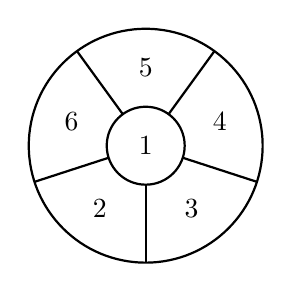
\begin{tikzpicture}[>=stealth,scale=0.9]
  \def\rIn{0.55}
  \def\rOut{1.65}
  % Circles
  \draw[thick] (0,0) circle (\rIn);
  \draw[thick] (0,0) circle (\rOut);
  
  % Radial lines
  \foreach \ang in {54, 126, 198, 270, 342} {
    \draw[thick] (\ang:\rIn) -- (\ang:\rOut);
  }
  
  % Labels
  \node at (0,0) {$1$};
  \node at (234:1.1) {$2$};
  \node at (306:1.1) {$3$};
  \node at (18:1.1) {$4$};
  \node at (90:1.1) {$5$};
  \node at (162:1.1) {$6$};
\end{tikzpicture}
\end{center}
\nopagebreak[4]
\Needspace{4\baselineskip}
\textbf{解析}
\nopagebreak[4]
\begin{center}% 2003 年辽宁卷第 15 题：花圃 6 个部分示意图
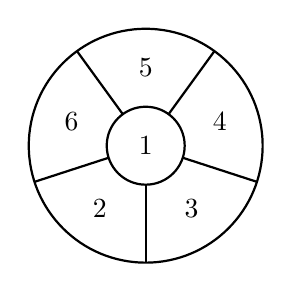
\begin{tikzpicture}[>=stealth,scale=0.9]
  \def\rIn{0.55}
  \def\rOut{1.65}
  % Circles
  \draw[thick] (0,0) circle (\rIn);
  \draw[thick] (0,0) circle (\rOut);
  
  % Radial lines
  \foreach \ang in {54, 126, 198, 270, 342} {
    \draw[thick] (\ang:\rIn) -- (\ang:\rOut);
  }
  
  % Labels
  \node at (0,0) {$1$};
  \node at (234:1.1) {$2$};
  \node at (306:1.1) {$3$};
  \node at (18:1.1) {$4$};
  \node at (90:1.1) {$5$};
  \node at (162:1.1) {$6$};
\end{tikzpicture}
\end{center}
\nopagebreak[4]
花圃分为中心部分 1 和外围 5 个环形部分 2, 3, 4, 5, 6。
共有 4 种不同颜色的花，相邻部分颜色不同：
1. 中心部分 1 与外围 5 个部分都相邻，先给部分 1 涂色，有 4 种选择；
2. 涂完部分 1 后，还剩 3 种颜色可供外围环形的 5 个扇区使用，且外围相邻两扇区颜色不同。
设用 3 种颜色对长度为 5 的环进行染色（环状染色色数多项式）：
\Needspace{5\baselineskip}
由容斥原理或递推关系，用 $k$ 种颜色染长度为 $n$ 的环，相邻不同色，染色方案数为：
\nopagebreak[4]
\[P(k, n) = (k - 1)^n + (-1)^n (k - 1).\]
\Needspace{5\baselineskip}
代入 $k = 3, n = 5$：
\nopagebreak[4]
\[P(3, 5) = (3 - 1)^5 + (-1)^5 (3 - 1) = 2^5 - 2 = 32 - 2 = 30.\]
\Needspace{5\baselineskip}
因此，不同的栽种方法总数为：
\nopagebreak[4]
\[N = 4 \times P(3, 5) = 4 \times 30 = 120 \text{ \text{种}}.\]

\gkanswer{答案：120}

\end{answer}
\begin{answer}
\gksolhead{16}{}

\textbf{题目}：

对于四面体 $ABCD$，给出下列四个命题：
① 若 $AB = AC$，$BD = CD$，则 $BC \perp AD$；
② 若 $AB = CD$，$AC = BD$，则 $BC \perp AD$；
③ 若 $AB \perp AC$，$BD \perp CD$，则 $BC \perp AD$；
④ 若 $AB \perp CD$，$AC \perp BD$，则 $BC \perp AD$．
其中真命题的序号是 $\underline{\hspace{2em}}$．（写出所有真命题的序号）

\Needspace{4\baselineskip}
\textbf{解析}

对四面体 $ABCD$ 的四个命题逐一分析：
\begin{itemize}
\item \textbf{命题①}：取 $BC$ 的中点 $M$，连接 $AM, DM$。因为 $AB = AC$，所以 $\triangle ABC$ 为等腰三角形，$AM \perp BC$；因为 $BD = CD$，所以 $\triangle BCD$ 为等腰三角形，$DM \perp BC$。由于 $AM \cap DM = M$，所以 $BC \perp \text{\text{平面} } AMD$。又 $AD \subset \text{\text{平面} } AMD$，故 $BC \perp AD$。命题①为真命题。
\item \textbf{命题②}：取特殊位置，当四面体 $ABCD$ 为等面四面体时，各面对角线相等；反例表明对棱相等的四面体，其对棱一般互不垂直，故②为假命题。
\item \textbf{命题③}：在直角三角形 $\triangle ABC$ 中 $\angle BAC = 90^\circ$，在 $\triangle BCD$ 中 $\angle BDC = 90^\circ$。将两直角三角形绕 $BC$ 旋转到任意空间夹角，对棱 $BC$ 与 $AD$ 一般不垂直，故③为假命题。
\item \textbf{命题④}：设 $\vec{BC} = \vec{AC} - \vec{AB}$。由已知 $AB \perp CD \implies \vec{AB} \cdot \vec{CD} = 0$，由 $AC \perp BD \implies \vec{AC} \cdot \vec{BD} = 0$。
\end{itemize}
\Needspace{5\baselineskip}
  注意到：
\nopagebreak[4]
\[\vec{BC} \cdot \vec{AD} = (\vec{AC} - \vec{AB}) \cdot \vec{AD} = \vec{AC} \cdot \vec{AD} - \vec{AB} \cdot \vec{AD}.\]
\Needspace{5\baselineskip}
  又 $\vec{AD} = \vec{AB} + \vec{BD} = \vec{AC} + \vec{CD}$，代入得：
\nopagebreak[4]
\[\vec{AC} \cdot \vec{AD} = \vec{AC} \cdot (\vec{AB} + \vec{BD}) = \vec{AC} \cdot \vec{AB} + \vec{AC} \cdot \vec{BD} = \vec{AC} \cdot \vec{AB} + 0 = \vec{AC} \cdot \vec{AB},\]
\nopagebreak[4]
\[\vec{AB} \cdot \vec{AD} = \vec{AB} \cdot (\vec{AC} + \vec{CD}) = \vec{AB} \cdot \vec{AC} + \vec{AB} \cdot \vec{CD} = \vec{AB} \cdot \vec{AC} + 0 = \vec{AB} \cdot \vec{AC}.\]
\Needspace{5\baselineskip}
  两式相减得：
\nopagebreak[4]
\[\vec{BC} \cdot \vec{AD} = \vec{AC} \cdot \vec{AB} - \vec{AB} \cdot \vec{AC} = 0.\]
  故 $BC \perp AD$。命题④为真命题。

综上所述，真命题的序号是 ①④。

\gkanswer{答案：①④}

\end{answer}
\begin{answer}
\gksolhead{17}{}

\textbf{题目}：

已知正四棱柱 $ABCD - A_1B_1C_1D_1$，$AB = 1$，$AA_1 = 2$，$E$ 为 $CC_1$ 中点，$F$ 为 $BD_1$ 中点．
(1) 证明：$EF$ 为 $BD_1$ 与 $CC_1$ 的公垂线；
(2) 求点 $D_1$ 到面 $BDE$ 的距离．
\nopagebreak[4]
\begin{center}% 2003 年辽宁卷第 17 题：正四棱柱立体几何图
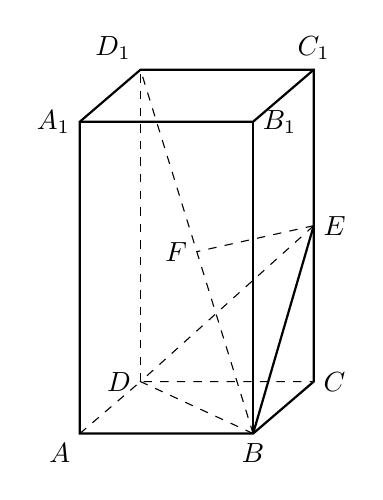
\begin{tikzpicture}[>=stealth,scale=1.1]
  % Coordinates
  \coordinate (A) at (0,0);
  \coordinate (B) at (2,0);
  \coordinate (C) at (2.7,0.6);
  \coordinate (D) at (0.7,0.6);

  \coordinate (A1) at (0,3.6);
  \coordinate (B1) at (2,3.6);
  \coordinate (C1) at (2.7,4.2);
  \coordinate (D1) at (0.7,4.2);

  \coordinate (E) at (2.7,2.4); % midpoint of CC1
  \coordinate (F) at (1.35,2.1); % midpoint of BD1

  % Solid edges
  \draw[thick] (A) -- (B) -- (C) -- (C1) -- (D1) -- (A1) -- cycle;
  \draw[thick] (A1) -- (B1) -- (C1);
  \draw[thick] (B) -- (B1);
  \draw[thick] (B) -- (E);

  % Dashed edges
  \draw[dashed] (A) -- (D) -- (C);
  \draw[dashed] (D) -- (D1);
  \draw[dashed] (B) -- (D1);
  \draw[dashed] (B) -- (D) -- (E);
  \draw[dashed] (E) -- (F);

  % Labels
  \node[below left] at (A) {$A$};
  \node[below] at (B) {$B$};
  \node[right] at (C) {$C$};
  \node[left] at (D) {$D$};
  \node[left] at (A1) {$A_1$};
  \node[right] at (B1) {$B_1$};
  \node[above] at (C1) {$C_1$};
  \node[above left] at (D1) {$D_1$};
  \node[right] at (E) {$E$};
  \node[left] at (F) {$F$};
\end{tikzpicture}
\end{center}
\nopagebreak[4]
\Needspace{4\baselineskip}
\textbf{解析}
\nopagebreak[4]
\begin{center}% 2003 年辽宁卷第 17 题：正四棱柱立体几何图
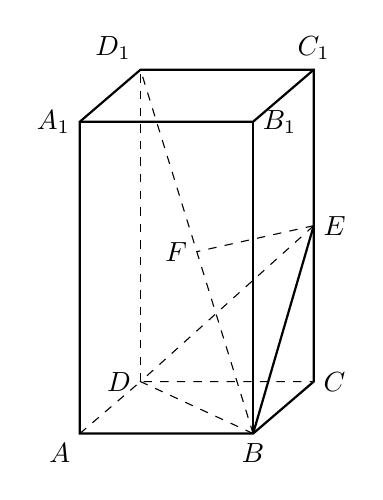
\begin{tikzpicture}[>=stealth,scale=1.1]
  % Coordinates
  \coordinate (A) at (0,0);
  \coordinate (B) at (2,0);
  \coordinate (C) at (2.7,0.6);
  \coordinate (D) at (0.7,0.6);

  \coordinate (A1) at (0,3.6);
  \coordinate (B1) at (2,3.6);
  \coordinate (C1) at (2.7,4.2);
  \coordinate (D1) at (0.7,4.2);

  \coordinate (E) at (2.7,2.4); % midpoint of CC1
  \coordinate (F) at (1.35,2.1); % midpoint of BD1

  % Solid edges
  \draw[thick] (A) -- (B) -- (C) -- (C1) -- (D1) -- (A1) -- cycle;
  \draw[thick] (A1) -- (B1) -- (C1);
  \draw[thick] (B) -- (B1);
  \draw[thick] (B) -- (E);

  % Dashed edges
  \draw[dashed] (A) -- (D) -- (C);
  \draw[dashed] (D) -- (D1);
  \draw[dashed] (B) -- (D1);
  \draw[dashed] (B) -- (D) -- (E);
  \draw[dashed] (E) -- (F);

  % Labels
  \node[below left] at (A) {$A$};
  \node[below] at (B) {$B$};
  \node[right] at (C) {$C$};
  \node[left] at (D) {$D$};
  \node[left] at (A1) {$A_1$};
  \node[right] at (B1) {$B_1$};
  \node[above] at (C1) {$C_1$};
  \node[above left] at (D1) {$D_1$};
  \node[right] at (E) {$E$};
  \node[left] at (F) {$F$};
\end{tikzpicture}
\end{center}
\nopagebreak[4]
在正四棱柱 $ABCD - A_1B_1C_1D_1$ 中，底面 $ABCD$ 为边长为 1 的正方形，侧棱长为 2 且垂直于底面。
\Needspace{5\baselineskip}
以 $D$ 为原点，$DA, DC, DD_1$ 所在直线分别为 $x, y, z$ 轴建立空间直角坐标系：
\nopagebreak[4]
\[D(0, 0, 0), \quad A(1, 0, 0), \quad B(1, 1, 0), \quad C(0, 1, 0),\]
\nopagebreak[4]
\[D_1(0, 0, 2), \quad A_1(1, 0, 2), \quad B_1(1, 1, 2), \quad C_1(0, 1, 2).\]
\Needspace{5\baselineskip}
因为 $E$ 为 $CC_1$ 中点，$F$ 为 $BD_1$ 中点，所以：
\nopagebreak[4]
\[E(0, 1, 1), \quad F\left(\frac{1+0}{2}, \frac{1+0}{2}, \frac{0+2}{2}\right) = \left(\frac{1}{2}, \frac{1}{2}, 1\right).\]

\gksubpart{(1)}

向量 $\vec{EF} = F - E = \left(\dfrac{1}{2}, -\dfrac{1}{2}, 0\right)$。
\Needspace{5\baselineskip}
直线 $CC_1$ 的方向向量为 $\vec{CC_1} = (0, 0, 2)$，数量积为：
\nopagebreak[4]
\[\vec{EF} \cdot \vec{CC_1} = \frac{1}{2} \times 0 + \left(-\frac{1}{2}\right) \times 0 + 0 \times 2 = 0 \implies EF \perp CC_1.\]
\Needspace{5\baselineskip}
直线 $BD_1$ 的方向向量为 $\vec{BD_1} = D_1 - B = (-1, -1, 2)$，数量积为：
\nopagebreak[4]
\[\vec{EF} \cdot \vec{BD_1} = \frac{1}{2} \times (-1) + \left(-\frac{1}{2}\right) \times (-1) + 0 \times 2 = -\frac{1}{2} + \frac{1}{2} = 0 \implies EF \perp BD_1.\]
又因为点 $E$ 在直线 $CC_1$ 上，点 $F$ 在直线 $BD_1$ 上，
所以 $EF$ 为 $BD_1$ 与 $CC_1$ 的公垂线。

\gksubpart{(2)}

\Needspace{5\baselineskip}
在平面 $BDE$ 中，已知：
\nopagebreak[4]
\[D(0, 0, 0), \quad B(1, 1, 0), \quad E(0, 1, 1).\]
向量 $\vec{DB} = (1, 1, 0)$，$\vec{DE} = (0, 1, 1)$。
\Needspace{5\baselineskip}
设平面 $BDE$ 的法向量为 $\vec{n} = (x, y, z)$，由 $\vec{n} \perp \vec{DB}$ 且 $\vec{n} \perp \vec{DE}$ 得：
\nopagebreak[4]
\[\begin{cases} x + y = 0, \\ y + z = 0. \end{cases}\]
取 $y = -1$，则 $x = 1, z = 1$。
故平面 $BDE$ 的一个法向量为 $\vec{n} = (1, -1, 1)$。
向量 $\vec{DD_1} = (0, 0, 2)$。
\Needspace{5\baselineskip}
点 $D_1$ 到平面 $BDE$ 的距离为：
\nopagebreak[4]
\[d = \frac{|\vec{DD_1} \cdot \vec{n}|}{|\vec{n}|} = \frac{|0 \times 1 + 0 \times (-1) + 2 \times 1|}{\sqrt{1^2 + (-1)^2 + 1^2}} = \frac{2}{\sqrt{3}} = \frac{2\sqrt{3}}{3}.\]

\gkanswer{答案（1）：证明见解析}

\gkanswer{答案（2）：$\dfrac{2\sqrt{3}}{3}$}

\end{answer}
\begin{answer}
\gksolhead{18}{}

\textbf{题目}：

已知函数 $f(x) = \sin(\omega x + \varphi)$（$\omega > 0$，$0 \le \varphi \le \pi$）是 $\mathbf{R}$ 上的偶函数，其图象关于点 $M\left(\dfrac{3\pi}{4}, 0\right)$ 对称，且在区间 $\left[0, \dfrac{\pi}{2}\right]$ 上是单调函数．求 $\omega$ 和 $\varphi$ 的值．

\Needspace{4\baselineskip}
\textbf{解析}

已知函数 $f(x) = \sin(\omega x + \varphi)$（$\omega > 0$，$0 \le \varphi \le \pi$）是 $\mathbf{R}$ 上的偶函数。
由偶函数性质可知 $f(0) = \pm 1$，即 $\sin\varphi = \pm 1$。
\Needspace{5\baselineskip}
结合 $0 \le \varphi \le \pi$，得：
\nopagebreak[4]
\[\varphi = \frac{\pi}{2}.\]
\Needspace{5\baselineskip}
此时：
\nopagebreak[4]
\[f(x) = \sin\left(\omega x + \frac{\pi}{2}\right) = \cos(\omega x).\]
\Needspace{5\baselineskip}
由题意，函数图象关于点 $M\left(\dfrac{3\pi}{4}, 0\right)$ 对称，所以：
\nopagebreak[4]
\[f\left(\frac{3\pi}{4}\right) = \cos\left(\frac{3\pi}{4}\omega\right) = 0.\]
\Needspace{5\baselineskip}
从而：
\nopagebreak[4]
\[\frac{3\pi}{4}\omega = k\pi + \frac{\pi}{2} = \frac{2k+1}{2}\pi \implies \omega = \frac{4k+2}{3} \quad (k \in \mathbf{Z}).\]
因为 $\omega > 0$，所以 $k \ge 0$。
\begin{itemize}
\item 当 $k = 0$ 时，$\omega = \dfrac{2}{3}$；
\item 当 $k = 1$ 时，$\omega = 2$；
\item 当 $k = 2$ 时，$\omega = \dfrac{10}{3}$；依此类推。
\end{itemize}
又已知函数 $f(x) = \cos(\omega x)$ 在区间 $\left[0, \dfrac{\pi}{2}\right]$ 上是单调函数。
余弦函数 $y = \cos u$ 从 $u = 0$ 开始的第一个单调递减区间为 $[0, \pi]$。
\Needspace{5\baselineskip}
因此，当 $x \in \left[0, \dfrac{\pi}{2}\right]$ 时，$\omega x \in \left[0, \dfrac{\omega\pi}{2}\right]$，要求函数单调，必须且只需：
\nopagebreak[4]
\[\frac{\omega\pi}{2} \le \pi \implies \omega \le 2.\]
由 $\omega > 0$ 且 $\omega = \dfrac{4k+2}{3}$，结合 $\omega \le 2$：
\begin{itemize}
\item 当 $k = 0$ 时，$\omega = \dfrac{2}{3} \le 2$，符合题意；
\item 当 $k = 1$ 时，$\omega = 2 \le 2$，符合题意；
\item 当 $k \ge 2$ 时，$\omega \ge \dfrac{10}{3} > 2$，在 $\left[0, \dfrac{\pi}{2}\right]$ 上不单调，舍去。
\end{itemize}

综上所述，$\varphi = \dfrac{\pi}{2}$，$\omega = \dfrac{2}{3}$ 或 $\omega = 2$。

\gkanswer{答案：$\varphi = \dfrac{\pi}{2}$，$\omega = \dfrac{2}{3}$ 或 $\omega = 2$}

\end{answer}
\begin{answer}
\gksolhead{19}{}

\textbf{题目}：

设 $a > 0$，求函数 $f(x) = \sqrt{x} - \ln(x + a)$，$x \in (0, +\infty)$ 的单调区间．

\Needspace{4\baselineskip}
\textbf{解析}

已知函数 $f(x) = \sqrt{x} - \ln(x + a)$，定义域为 $(0, +\infty)$，参数 $a > 0$。
\Needspace{5\baselineskip}
求导数：
\nopagebreak[4]
\[f'(x) = \frac{1}{2\sqrt{x}} - \frac{1}{x + a} = \frac{x + a - 2\sqrt{x}}{2\sqrt{x}(x + a)}.\]
因为 $x \in (0, +\infty)$ 且 $a > 0$，分母 $2\sqrt{x}(x + a) > 0$，所以 $f'(x)$ 的符号由分子决定。
令 $t = \sqrt{x} > 0$，则 $x = t^2$。
\Needspace{5\baselineskip}
分子关于 $t$ 的表达式为二次函数：
\nopagebreak[4]
\[g(t) = t^2 - 2t + a.\]
\Needspace{5\baselineskip}
判别式为：
\nopagebreak[4]
\[\Delta = (-2)^2 - 4a = 4(1 - a).\]
分情况讨论：

1. \textbf{当 $a \ge 1$ 时}：
   $\Delta = 4(1 - a) \le 0$。
   此时二次函数 $g(t) = (t - 1)^2 + a - 1 \ge 0$。
   特别地，当 $a > 1$ 时，$g(t) > 0$ 恒成立，即 $f'(x) > 0$ 在 $(0, +\infty)$ 上恒成立；
   当 $a = 1$ 时，$g(t) = (t - 1)^2 \ge 0$，仅在 $t = 1$（即 $x = 1$）处导数为 0。
   因此，当 $a \ge 1$ 时，函数 $f(x)$ 在 $(0, +\infty)$ 上严格单调递增。
   单调递增区间为 $(0, +\infty)$，无单调递减区间。

2. \textbf{当 $0 < a < 1$ 时}：
   $\Delta = 4(1 - a) > 0$。
\Needspace{5\baselineskip}
   方程 $t^2 - 2t + a = 0$ 有两个不同的正实根：
\nopagebreak[4]
\[t_1 = 1 - \sqrt{1 - a}, \quad t_2 = 1 + \sqrt{1 - a}.\]
   因为 $0 < a < 1$，所以 $0 < \sqrt{1 - a} < 1$，故 $0 < t_1 < 1 < t_2$。
\Needspace{5\baselineskip}
   对应到变量 $x = t^2$：
\nopagebreak[4]
\[x_1 = t_1^2 = (1 - \sqrt{1 - a})^2 = 2 - a - 2\sqrt{1 - a},\]
\nopagebreak[4]
\[x_2 = t_2^2 = (1 + \sqrt{1 - a})^2 = 2 - a + 2\sqrt{1 - a}.\]
\begin{itemize}
\item 当 $t \in (0, t_1)$ 即 $x \in (0, x_1)$ 时，$g(t) > 0 \implies f'(x) > 0$；
\item 当 $t \in (t_1, t_2)$ 即 $x \in (x_1, x_2)$ 时，$g(t) < 0 \implies f'(x) < 0$；
\item 当 $t \in (t_2, +\infty)$ 即 $x \in (x_2, +\infty)$ 时，$g(t) > 0 \implies f'(x) > 0$。
\end{itemize}
   因此：
\begin{itemize}
\item 函数的单调递增区间为：$(0, (1 - \sqrt{1 - a})^2]$ 和 $[(1 + \sqrt{1 - a})^2, +\infty)$；
\item 函数的单调递减区间为：$[(1 - \sqrt{1 - a})^2, (1 + \sqrt{1 - a})^2]$。
\end{itemize}

\gkanswer{答案：当 $a \ge 1$ 时，函数的单调递增区间为 $(0, +\infty)$，无单调递减区间；当 $0 < a < 1$ 时，函数的单调递增区间为 $(0, (1-\sqrt{1-a})^2]$ 和 $[(1+\sqrt{1-a})^2, +\infty)$，单调递减区间为 $[(1-\sqrt{1-a})^2, (1+\sqrt{1-a})^2]$。}

\end{answer}
\begin{answer}
\gksolhead{20}{}

\textbf{题目}：

A、B 两个代表队进行乒乓球对抗赛，每队三名队员，A 队队员是 $A_1, A_2, A_3$，B 队队员是 $B_1, B_2, B_3$，按以往多次比赛的统计，对阵队员之间胜负概率如下：

\begin{center}
\begin{tabular}{lll}
\toprule
对阵队员 & A 队队员胜的概率 & A 队队员负的概率 \\
\midrule
$A_1$ 对 $B_1$ & $\dfrac{2}{3}$ & $\dfrac{1}{3}$ \\
$A_2$ 对 $B_2$ & $\dfrac{2}{5}$ & $\dfrac{3}{5}$ \\
$A_3$ 对 $B_3$ & $\dfrac{2}{5}$ & $\dfrac{3}{5}$ \\
\bottomrule
\end{tabular}
\end{center}

现按表中对阵方式出场，每场胜队得 1 分，负队得 0 分，设 A 队、B 队最后所得总分分别为 $\xi$、$\eta$．
(1) 求 $\xi$、$\eta$ 的概率分布；
(2) 求 $E\xi$，$E\eta$．

\Needspace{4\baselineskip}
\textbf{解析}

\gksubpart{(1)}

设事件 $C_i$ 表示第 $i$ 场比赛 A 队队员胜出（$i = 1, 2, 3$），则 $C_1, C_2, C_3$ 相互独立。
\Needspace{5\baselineskip}
由题设概率：
\nopagebreak[4]
\[P(C_1) = \frac{2}{3}, \quad P(\bar{C}_1) = \frac{1}{3};\]
\nopagebreak[4]
\[P(C_2) = \frac{2}{5}, \quad P(\bar{C}_2) = \frac{3}{5};\]
\nopagebreak[4]
\[P(C_3) = \frac{2}{5}, \quad P(\bar{C}_3) = \frac{3}{5}.\]
A 队总分 $\xi$ 的可能取值为 $0, 1, 2, 3$：
\begin{itemize}
\item $P(\xi = 0) = P(\bar{C}_1 \bar{C}_2 \bar{C}_3) = \dfrac{1}{3} \times \dfrac{3}{5} \times \dfrac{3}{5} = \dfrac{9}{75} = \dfrac{3}{25}$；
\item $P(\xi = 1) = P(C_1 \bar{C}_2 \bar{C}_3) + P(\bar{C}_1 C_2 \bar{C}_3) + P(\bar{C}_1 \bar{C}_2 C_3)$
\end{itemize}
\nopagebreak[4]
\[= \frac{2}{3} \times \frac{3}{5} \times \frac{3}{5} + \frac{1}{3} \times \frac{2}{5} \times \frac{3}{5} + \frac{1}{3} \times \frac{3}{5} \times \frac{2}{5} = \frac{18 + 6 + 6}{75} = \frac{30}{75} = \frac{2}{5};\]
\begin{itemize}
\item $P(\xi = 2) = P(C_1 C_2 \bar{C}_3) + P(C_1 \bar{C}_2 C_3) + P(\bar{C}_1 C_2 C_3)$
\end{itemize}
\nopagebreak[4]
\[= \frac{2}{3} \times \frac{2}{5} \times \frac{3}{5} + \frac{2}{3} \times \frac{3}{5} \times \frac{2}{5} + \frac{1}{3} \times \frac{2}{5} \times \frac{2}{5} = \frac{12 + 12 + 4}{75} = \frac{28}{75};\]
\begin{itemize}
\item $P(\xi = 3) = P(C_1 C_2 C_3) = \dfrac{2}{3} \times \dfrac{2}{5} \times \dfrac{2}{5} = \dfrac{8}{75}$。
\end{itemize}

因为每场比赛必有一队胜得 1 分、另一队负得 0 分，总比赛场数为 3，所以总分满足 $\xi + \eta = 3 \implies \eta = 3 - \xi$。
B 队总分 $\eta$ 的可能取值也为 $0, 1, 2, 3$：
\begin{itemize}
\item $P(\eta = 0) = P(\xi = 3) = \dfrac{8}{75}$；
\item $P(\eta = 1) = P(\xi = 2) = \dfrac{28}{75}$；
\item $P(\eta = 2) = P(\xi = 1) = \dfrac{30}{75} = \dfrac{2}{5}$；
\item $P(\eta = 3) = P(\xi = 0) = \dfrac{9}{75} = \dfrac{3}{25}$。
\end{itemize}

\gksubpart{(2)}

记 $\xi_i$ 为第 $i$ 场比赛 A 队的得分，则 $\xi = \xi_1 + \xi_2 + \xi_3$。
\Needspace{5\baselineskip}
各场得分的数学期望为：
\nopagebreak[4]
\[E(\xi_1) = 1 \times P(C_1) = \frac{2}{3}, \quad E(\xi_2) = \frac{2}{5}, \quad E(\xi_3) = \frac{2}{5}.\]
\Needspace{5\baselineskip}
由数学期望的线性性质：
\nopagebreak[4]
\[E\xi = E(\xi_1) + E(\xi_2) + E(\xi_3) = \frac{2}{3} + \frac{2}{5} + \frac{2}{5} = \frac{2}{3} + \frac{4}{5} = \frac{22}{15}.\]
\Needspace{5\baselineskip}
因为 $\eta = 3 - \xi$，所以：
\nopagebreak[4]
\[E\eta = 3 - E\xi = 3 - \frac{22}{15} = \frac{23}{15}.\]

\gkanswer{答案（1）：$\xi$ 的概率分布为 $P(\xi=0)=\dfrac{3}{25}$，$P(\xi=1)=\dfrac{2}{5}$，$P(\xi=2)=\dfrac{28}{75}$，$P(\xi=3)=\dfrac{8}{75}$；$\eta$ 的概率分布为 $P(\eta=0)=\dfrac{8}{75}$，$P(\eta=1)=\dfrac{28}{75}$，$P(\eta=2)=\dfrac{2}{5}$，$P(\eta=3)=\dfrac{3}{25}$}

\gkanswer{答案（2）：$E\xi = \dfrac{22}{15}$，$E\eta = \dfrac{23}{15}$}

\end{answer}
\begin{answer}
\gksolhead{21}{}

\textbf{题目}：

设 $a_0$ 为常数，且 $a_n = 3^{n-1} - 2a_{n-1}$ ($n \in \mathbf{N}^*$)．
(1) 证明对任意 $n \ge 1$，$a_n = \dfrac{1}{5}[3^n + (-1)^{n-1} \cdot 2^n] + (-1)^n \cdot 2^n a_0$；
(2) 假设对任意 $n \ge 1$ 有 $a_n > a_{n-1}$，求 $a_0$ 的取值范围．

\Needspace{4\baselineskip}
\textbf{解析}

\gksubpart{(1)}

用数学归纳法证明对任意 $n \ge 1$ 成立：
1. 当 $n = 1$ 时：
   左边 $= a_1 = 3^{1-1} - 2a_0 = 1 - 2a_0$；
   右边 $= \dfrac{1}{5}[3^1 + (-1)^0 \cdot 2^1] + (-1)^1 \cdot 2^1 a_0 = \dfrac{1}{5}[3 + 2] - 2a_0 = 1 - 2a_0$。
   左边等于右边，等式成立。
\Needspace{5\baselineskip}
2. 假设当 $n = k$ ($k \ge 1$) 时等式成立，即：
\nopagebreak[4]
\[a_k = \frac{1}{5}[3^k + (-1)^{k-1} \cdot 2^k] + (-1)^k \cdot 2^k a_0.\]
\Needspace{5\baselineskip}
   那么当 $n = k + 1$ 时，由递推关系 $a_{k+1} = 3^k - 2a_k$，代入归纳假设：
\nopagebreak[4]
\[\begin{aligned}
a_{k+1} &= 3^k - 2\left(\frac{1}{5}[3^k + (-1)^{k-1} \cdot 2^k] + (-1)^k \cdot 2^k a_0\right) \\
&= 3^k - \frac{2}{5}\cdot 3^k - \frac{1}{5}(-1)^{k-1}\cdot 2^{k+1} - (-1)^k \cdot 2^{k+1} a_0 \\
&= \frac{3}{5}\cdot 3^k + \frac{1}{5}(-1)^k \cdot 2^{k+1} + (-1)^{k+1} \cdot 2^{k+1} a_0 \\
&= \frac{1}{5}[3^{k+1} + (-1)^k \cdot 2^{k+1}] + (-1)^{k+1} \cdot 2^{k+1} a_0.
\end{aligned}\]
   即当 $n = k + 1$ 时等式也成立。
由 1 和 2 可知，对任意正整数 $n \ge 1$ 命题成立。

\gksubpart{(2)}

\Needspace{5\baselineskip}
由题设 $a_n > a_{n-1}$ 对任意 $n \ge 1$ 恒成立，结合递推关系 $a_n = 3^{n-1} - 2a_{n-1}$：
\nopagebreak[4]
\[a_n - a_{n-1} = 3^{n-1} - 3a_{n-1} > 0 \iff a_{n-1} < 3^{n-2}.\]
\Needspace{5\baselineskip}
令 $m = n - 1 \ge 0$，则对任意非负整数 $m \ge 0$，都有：
\nopagebreak[4]
\[a_m < 3^{m-1}.\]
\begin{itemize}
\item 当 $m = 0$ 时，直接得：
\end{itemize}
\nopagebreak[4]
\[a_0 < 3^{-1} = \frac{1}{3}.\]
\begin{itemize}
\item 当 $m \ge 1$ 时，代入 (1) 的通项公式：
\end{itemize}
\nopagebreak[4]
\[\frac{1}{5}[3^m + (-1)^{m-1} \cdot 2^m] + (-1)^m \cdot 2^m a_0 < 3^{m-1} = \frac{1}{3}\cdot 3^m.\]
\Needspace{5\baselineskip}
  移项整理：
\nopagebreak[4]
\[(-1)^m \cdot 2^m a_0 < \left(\frac{1}{3} - \frac{1}{5}\right) 3^m - \frac{1}{5}(-1)^{m-1}\cdot 2^m = \frac{2}{15}\cdot 3^m + \frac{1}{5}(-1)^m \cdot 2^m.\]
\Needspace{5\baselineskip}
  两边同除以 $2^m$：
\nopagebreak[4]
\[(-1)^m a_0 < \frac{2}{15}\left(\frac{3}{2}\right)^m + \frac{1}{5}(-1)^m \iff (-1)^m \left(a_0 - \frac{1}{5}\right) < \frac{2}{15}\left(\frac{3}{2}\right)^m.\]
分 $m$ 的奇偶性讨论：
\Needspace{5\baselineskip}
1. 当 $m$ 为偶数时，$(-1)^m = 1$：
\nopagebreak[4]
\[a_0 - \frac{1}{5} < \frac{2}{15}\left(\frac{3}{2}\right)^m \iff a_0 < \frac{1}{5} + \frac{2}{15}\left(\frac{3}{2}\right)^m.\]
\Needspace{5\baselineskip}
   因为对于偶数 $m \ge 0$，$\left(\dfrac{3}{2}\right)^m \ge 1$，右边的最小值为当 $m = 0$ 时的值：
\nopagebreak[4]
\[\frac{1}{5} + \frac{2}{15} = \frac{1}{3}.\]
   因此必须 $a_0 < \dfrac{1}{3}$。
\Needspace{5\baselineskip}
2. 当 $m$ 为奇数时，$(-1)^m = -1$：
\nopagebreak[4]
\[-\left(a_0 - \frac{1}{5}\right) < \frac{2}{15}\left(\frac{3}{2}\right)^m \iff a_0 > \frac{1}{5} - \frac{2}{15}\left(\frac{3}{2}\right)^m.\]
   考查右边函数 $h(m) = \dfrac{1}{5} - \dfrac{2}{15}\left(\dfrac{3}{2}\right)^m$：
   随着奇数 $m$ 增大，$\left(\dfrac{3}{2}\right)^m$ 严格递增，$h(m)$ 严格递减。
\Needspace{5\baselineskip}
   因此在正奇数集合 $\{1, 3, 5, \cdots\}$ 中，最大值在 $m = 1$ 处取得：
\nopagebreak[4]
\[h(1) = \frac{1}{5} - \frac{2}{15} \times \frac{3}{2} = \frac{1}{5} - \frac{1}{5} = 0.\]
\Needspace{5\baselineskip}
   要使不等式对所有奇数恒成立，必须且只需：
\nopagebreak[4]
\[a_0 > 0.\]

综合上述偶数与奇数条件，$a_0$ 的取值范围为 $\left(0, \dfrac{1}{3}\right)$。

\gkanswer{答案（1）：证明见解析}

\gkanswer{答案（2）：$\left(0, \dfrac{1}{3}\right)$}

\end{answer}
\begin{answer}
\gksolhead{22}{}

\textbf{题目}：

已知常数 $a > 0$，向量 $\vec{c} = (0, a)$，$\vec{i} = (1, 0)$．经过原点 $O$ 以 $\vec{c} + \lambda\vec{i}$ 为方向向量的直线与经过定点 $A(0, a)$ 以 $\vec{i} - 2\lambda\vec{c}$ 为方向向量的直线相交于 $P$，其中 $\lambda \in \mathbf{R}$．试问：是否存在两个定点 $E$、$F$，使得 $|PE| + |PF|$ 为定值．若存在，求出 $E$、$F$ 的坐标；若不存在，说明理由．

\Needspace{4\baselineskip}
\textbf{解析}

已知向量 $\vec{c} = (0, a)$，$\vec{i} = (1, 0)$，其中 $a > 0$。
\begin{itemize}
\item 直线 $l_1$ 经过原点 $O(0, 0)$，方向向量为 $\vec{c} + \lambda\vec{i} = (\lambda, a)$。
\end{itemize}
\Needspace{5\baselineskip}
  当 $\lambda \ne 0$ 时，直线的斜率为 $\dfrac{a}{\lambda}$，方程为：
\nopagebreak[4]
\[y = \frac{a}{\lambda} x \iff ax - \lambda y = 0.\]
  当 $\lambda = 0$ 时，方向向量为 $(0, a)$，直线为 $y$ 轴（$x = 0$），也满足上式。
\begin{itemize}
\item 直线 $l_2$ 经过定点 $A(0, a)$，方向向量为 $\vec{i} - 2\lambda\vec{c} = (1, -2\lambda a)$。
\end{itemize}
\Needspace{5\baselineskip}
  直线的斜率为 $-2\lambda a$，方程为：
\nopagebreak[4]
\[y - a = -2\lambda a x \iff 2\lambda a x + y - a = 0.\]
设直线 $l_1$ 与 $l_2$ 相交于点 $P(x, y)$。
由 $ax - \lambda y = 0$：
当 $y \ne 0$ 时，$\lambda = \dfrac{ax}{y}$。
\Needspace{5\baselineskip}
将其代入 $l_2$ 的方程中：
\nopagebreak[4]
\[2\left(\frac{ax}{y}\right) a x + y - a = 0 \implies \frac{2a^2 x^2}{y} + y - a = 0.\]
\Needspace{5\baselineskip}
两边同乘以 $y$ 并整理：
\nopagebreak[4]
\[2a^2 x^2 + y^2 - ay = 0.\]
\Needspace{5\baselineskip}
配方得：
\nopagebreak[4]
\[2a^2 x^2 + \left(y - \frac{a}{2}\right)^2 = \frac{a^2}{4}.\]
\Needspace{5\baselineskip}
两边同除以 $\dfrac{a^2}{4}$：
\nopagebreak[4]
\[\frac{x^2}{\dfrac{1}{8}} + \frac{\left(y - \dfrac{a}{2}\right)^2}{\dfrac{a^2}{4}} = 1.\]
（检验 $\lambda = 0$ 时，交点为 $(0, a)$，满足方程；当 $\lambda \to \infty$ 时交点趋近 $(0, 0)$）。
此方程表示中心在 $\left(0, \dfrac{a}{2}\right)$ 的二次曲线，根据椭圆第一定义，存在两个定点 $E, F$ 使得 $|PE| + |PF|$ 为定值。
比较两分母 $\dfrac{a^2}{4}$ 与 $\dfrac{1}{8}$ 的大小：

1. 当 $\dfrac{a^2}{4} > \dfrac{1}{8}$，即 $a > \dfrac{\sqrt{2}}{2}$ 时：
   曲线是长轴在直线 $x = 0$ 上的椭圆。
\Needspace{5\baselineskip}
   长半轴长为 $A = \dfrac{a}{2}$，半焦距为：
\nopagebreak[4]
\[c_0 = \sqrt{\frac{a^2}{4} - \frac{1}{8}} = \frac{\sqrt{4a^2 - 2}}{4}.\]
\Needspace{5\baselineskip}
   焦点在 $y$ 轴上，坐标为：
\nopagebreak[4]
\[E\left(0, \frac{a}{2} - \frac{\sqrt{4a^2 - 2}}{4}\right), \quad F\left(0, \frac{a}{2} + \frac{\sqrt{4a^2 - 2}}{4}\right).\]
   此时 $|PE| + |PF| = 2A = a$ 为定值。

2. 当 $\dfrac{a^2}{4} = \dfrac{1}{8}$，即 $a = \dfrac{\sqrt{2}}{2}$ 时：
   方程化为 $x^2 + \left(y - \dfrac{\sqrt{2}}{4}\right)^2 = \dfrac{1}{8}$，轨迹为圆。
   两焦点重合于圆心 $\left(0, \dfrac{\sqrt{2}}{4}\right)$，取 $E = F = \left(0, \dfrac{\sqrt{2}}{4}\right)$，
   此时 $|PE| + |PF| = 2|PE| = 2 \times \dfrac{\sqrt{2}}{4} = \dfrac{\sqrt{2}}{2}$ 为定值。

3. 当 $\dfrac{a^2}{4} < \dfrac{1}{8}$，即 $0 < a < \dfrac{\sqrt{2}}{2}$ 时：
   曲线是长轴在直线 $y = \dfrac{a}{2}$ 上的椭圆。
\Needspace{5\baselineskip}
   长半轴长为 $A = \dfrac{\sqrt{2}}{4}$，半焦距为：
\nopagebreak[4]
\[c_0 = \sqrt{\frac{1}{8} - \frac{a^2}{4}} = \frac{\sqrt{2 - 4a^2}}{4}.\]
\Needspace{5\baselineskip}
   焦点坐标为：
\nopagebreak[4]
\[E\left(-\frac{\sqrt{2 - 4a^2}}{4}, \frac{a}{2}\right), \quad F\left(\frac{\sqrt{2 - 4a^2}}{4}, \frac{a}{2}\right).\]
   此时 $|PE| + |PF| = 2A = \dfrac{\sqrt{2}}{2}$ 为定值。

\gkanswer{答案：存在。当 $a > \dfrac{\sqrt{2}}{2}$ 时，$E\left(0, \dfrac{a}{2} - \dfrac{\sqrt{4a^2 - 2}}{4}\right)$，$F\left(0, \dfrac{a}{2} + \dfrac{\sqrt{4a^2 - 2}}{4}\right)$，定值为 $a$；当 $a = \dfrac{\sqrt{2}}{2}$ 时，$E, F$ 重合于点 $\left(0, \dfrac{\sqrt{2}}{4}\right)$，定值为 $\dfrac{\sqrt{2}}{2}$；当 $0 < a < \dfrac{\sqrt{2}}{2}$ 时，$E\left(-\dfrac{\sqrt{2 - 4a^2}}{4}, \dfrac{a}{2}\right)$，$F\left(\dfrac{\sqrt{2 - 4a^2}}{4}, \dfrac{a}{2}\right)$，定值为 $\dfrac{\sqrt{2}}{2}$。}

\end{answer}